\chapter{Introduction to Hypothesis Testing \label{chapter:hypothesistesting}}

Hypothesis testing is a central idea underpinning much of the analysis in the clinical and biomedical research literature\footnote{I should state that there is still a lot of controversy around the whole idea of hypothesis testing and whether $p$-values should be used at all, etc.}. There are multiple approaches to hypothesis testing, but the most common is \textbf{null hypothesis testing}, which was developed by the statistician R.A. Fisher. In null hypothesis testing, one creates a model of how the data should look under default conditions and then quantifies the observed data's deviation from that model using a \textbf{test statistic}. If the test statistic is large enough, it means there is evidence that the default position is incorrect. 

The statisticians Jerzy Neyman and Karl Pearson developed a different approach to hypothesis testing based on the idea of \textbf{model comparison}. In their approach, one sets up different models and then quantifies each model's fit to the data; the hypothesis test is used to see whether one model's fit to the data is significantly better than another's. We see the Neyman-Pearson philosophy reflected in techniques such as power calculations and likelihood ratio tests. 

Most of the basic hypothesis tests we learn in introductory biostatistics courses (T-tests, chi-squared tests, etc.) follow Fisher's approach. We will focus on null hypothesis testing in this chapter and explore other ideas in subsequent chapters. 

%%%%%%%%%%%%%%%%%%%%%%%%%%%%%%%%%%%%%%%%%%%%%%%%%%%%%%%%%%%%%%%%%%%%%%%%%%%%%%%%

\section{Basic Steps of a Hypothesis Test}

\begin{enumerate}
\item \textit{State the \textbf{null hypothesis}}. The null hypothesis corresponds to the default, or baseline, position; for our example, the null hypothesis might be, ``The events `has mutation' and `has cancer' are statistically independent.'' The \textbf{alternative hypothesis} is the hypothesis that is contrary to the null; for our example, it might be, ``The events `has mutation' and `has cancer' are not statistically independent.''
\item \textit{List statistical {assumptions}}. All hypothesis tests make one or more assumptions about the data, and it's important to state them clearly. For example, \textbf{parametric} hypothesis tests assume the data follow a particular probability distribution under the null, while \textbf{nonparametric} tests do not make this assumption.
\item \textit{Decide on an appropriate test and test statistic}. The \textbf{test statistic} quantifies the degree of deviation of the observed data from what one would expect under the null hypothesis\footnote{Some definitions: A \textbf{statistic} is just some quantity that summarizes a set of data, or gives some information about the value of a parameter. A \textbf{sufficient statistic} is a statistic that gives the maximum amount of information about a parameter that can possibly be obtained from the sample data.}. 
\item \textit{Derive the distribution of the test statistic under the null}. This is called the \textbf{null distribution}.
\item \textit{Select a {significance level} under which you'll reject the null}. The \textbf{significance level}, usually written as $\alpha$, is the probability of a type I error. A type I error is committed when one rejects the null even though it is true (false positive result). 
\item \textit{Compute the observed value of the test statistic from the data.}
\item \textit{Decide whether or not to reject the null hypothesis.}
\end{enumerate}

%%%%%%%%%%%%%%%%%%%%%%%%%%%%%%%%%%%%%%%%%%%%%%%%%%%%%%%%%%%%%%%%%%%%%%%%%%%%%%%%%%%%%%

\section{The Z-Test}

A \textbf{Z-test} is a hypothesis test for which the null distribution is normal with known mean and standard deviation (i.e. known parameters $\mu$ and $\sigma$). It is most commonly used to compare the mean of a set of samples, $\overline{x}$, with a known population mean. It also appears in other contexts, such as significance tests of regression coefficients in generalized linear models (Chapter~\ref{chapter:glms}). 

\paragraph{Example: SBP in an Appalachian Town} The distribution of systolic blood pressure (SBP) among Caucasian males ages 55-64 in the United States is roughly normal with mean 139.75 mmHg and standard deviation 21.40 mmHg (Source: Int. J. Epidemiol. 2: 294-301, 1973). The following graph shows a normal distribution with those parameters.

\begin{center}
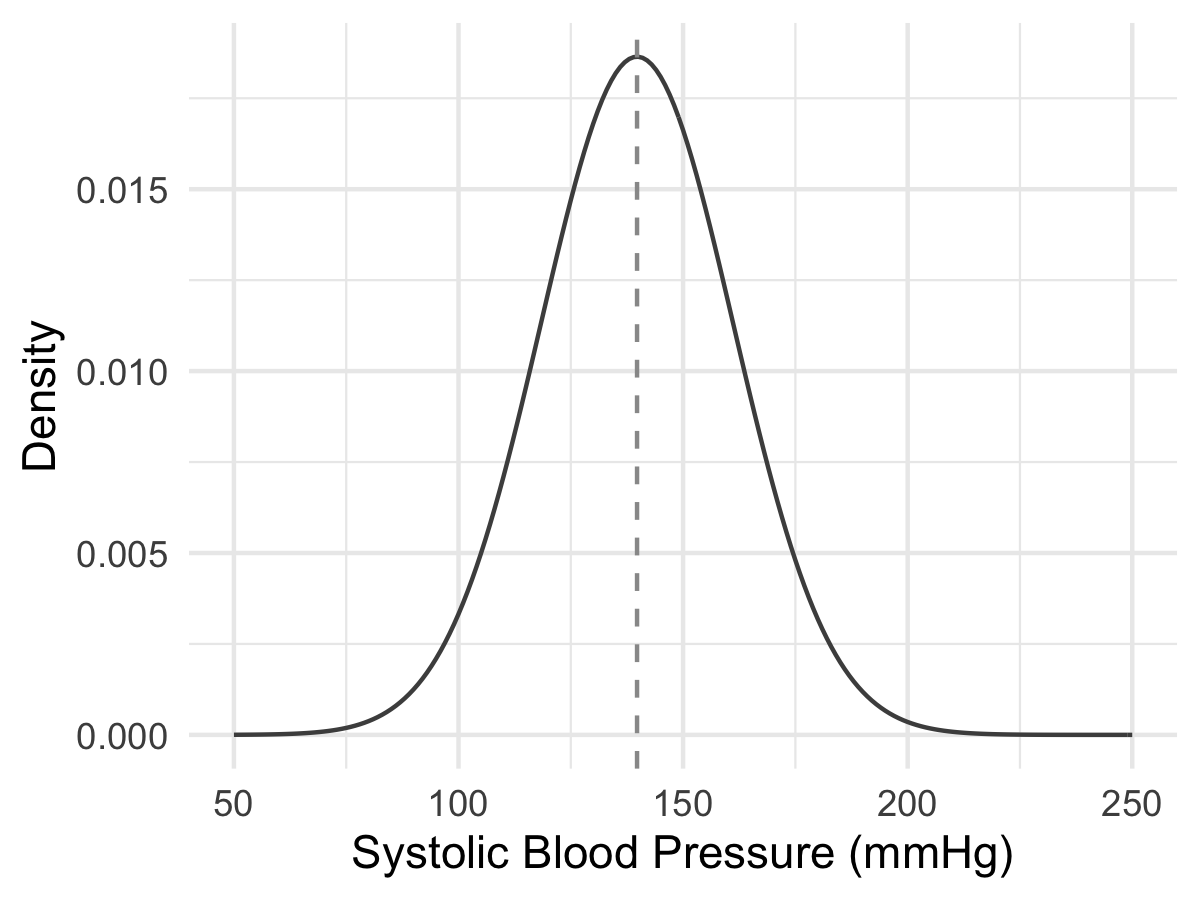
\includegraphics[width=0.7\textwidth]{img/hyp-z-test-example-00.png}
\end{center}

Here is a histogram of 10,000 data samples drawn independently from that distribution (i.e., what we would expect if we sampled the SBPs of 10,000 men from the United States at large):

\begin{center}
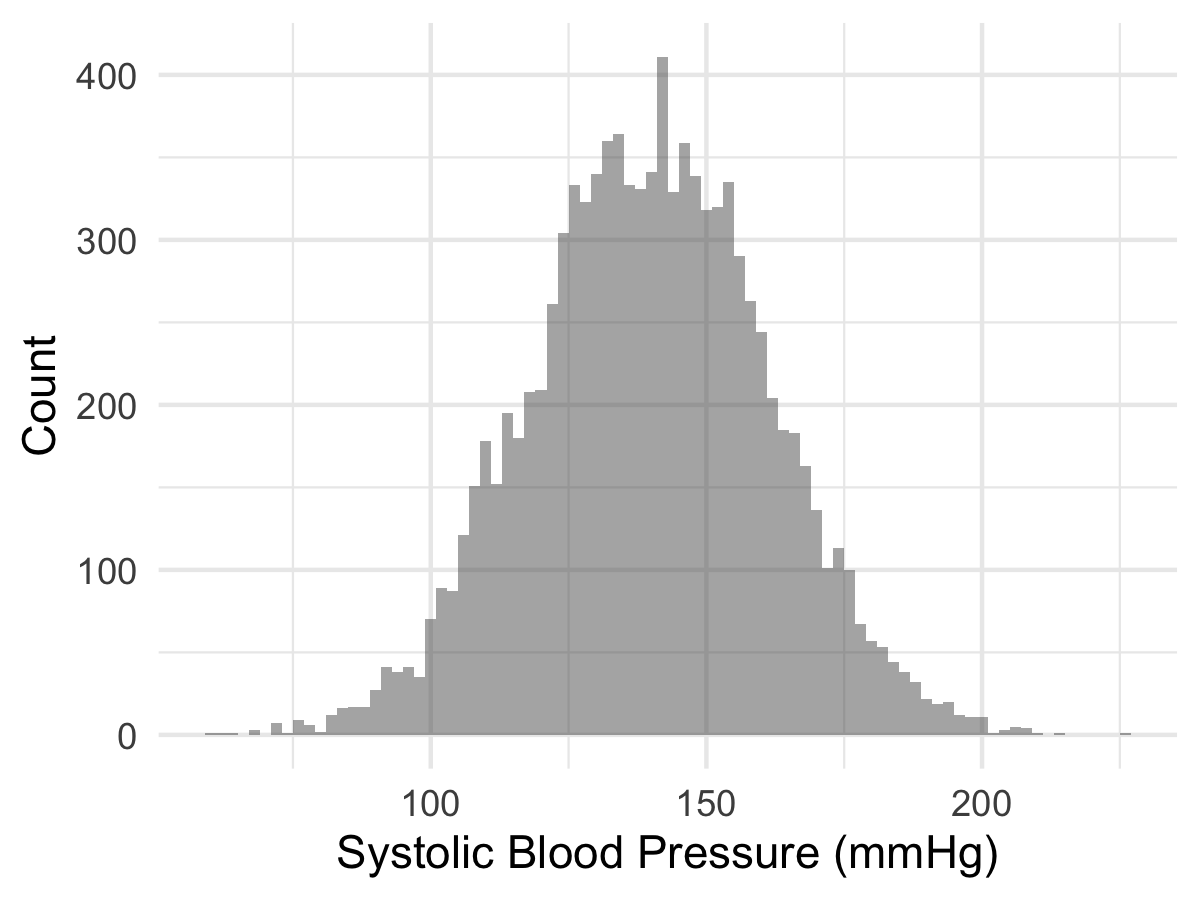
\includegraphics[width=0.7\textwidth]{img/hyp-z-test-example-0.png}
\end{center}

Now, assume some researchers find a small community in rural Appalachia and measure the SBP of 20 Caucasian males ages 55-64 there. Their mean SBP is 125.45 mmHg, illustrated by the red dashed line in the graph below.

\begin{center}
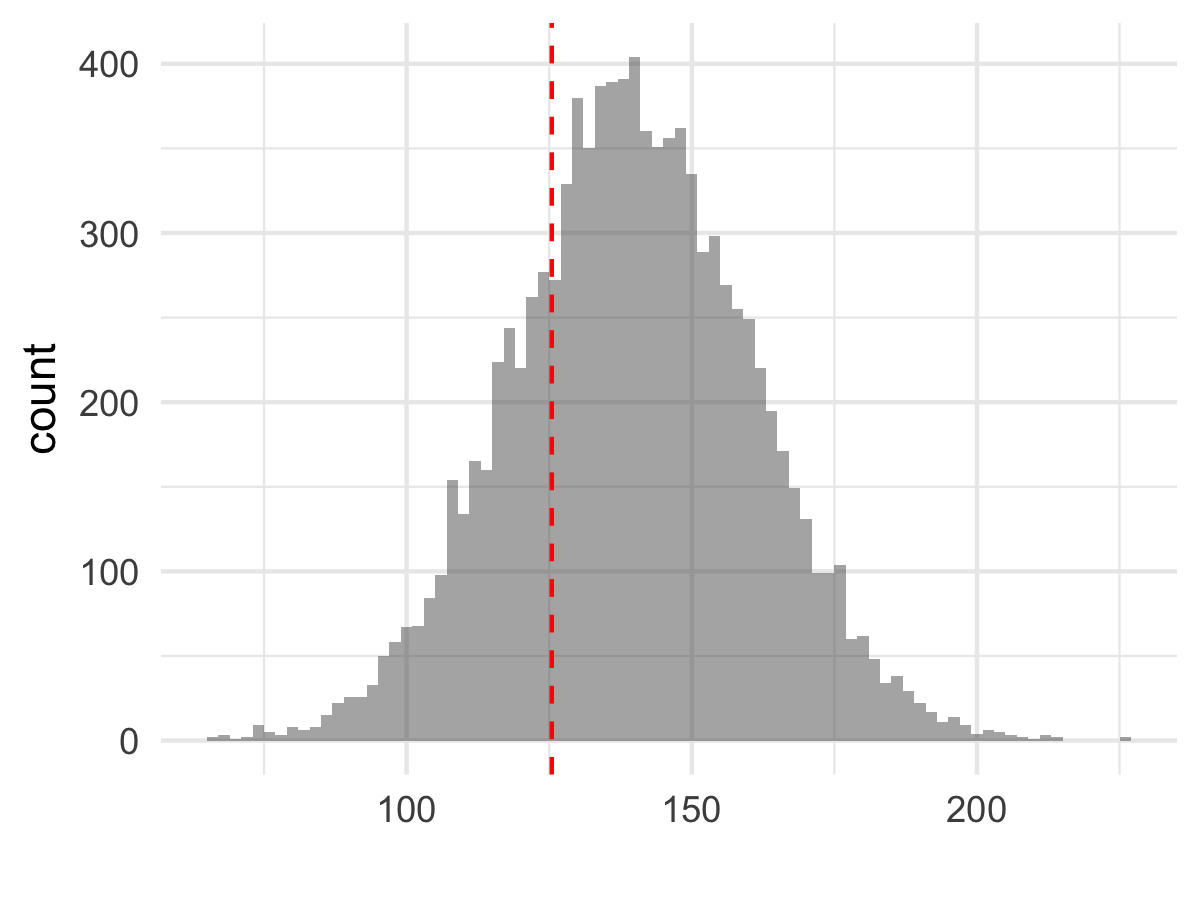
\includegraphics[width=0.7\textwidth]{img/hyp-z-test-example-1.png}
\end{center}

At first glance, this may not appear that unusual. After all, the red line is sort of near the center of the gray distribution, right? This analysis is flawed, however, because our 125.45 mmHg value isn't for one man - it's an average over 20 men. The distribution of the \textbf{sample mean}, $\overline{x}$, is different from that of each individual sample. 

To see this, imagine taking 20 samples from the gray distribution, taking their mean, and recording that value. Now repeat that process 10,000 times. If you do that, you get the \textbf{distribution of the sample mean},  which is skinnier than the gray distribution:
\begin{center}
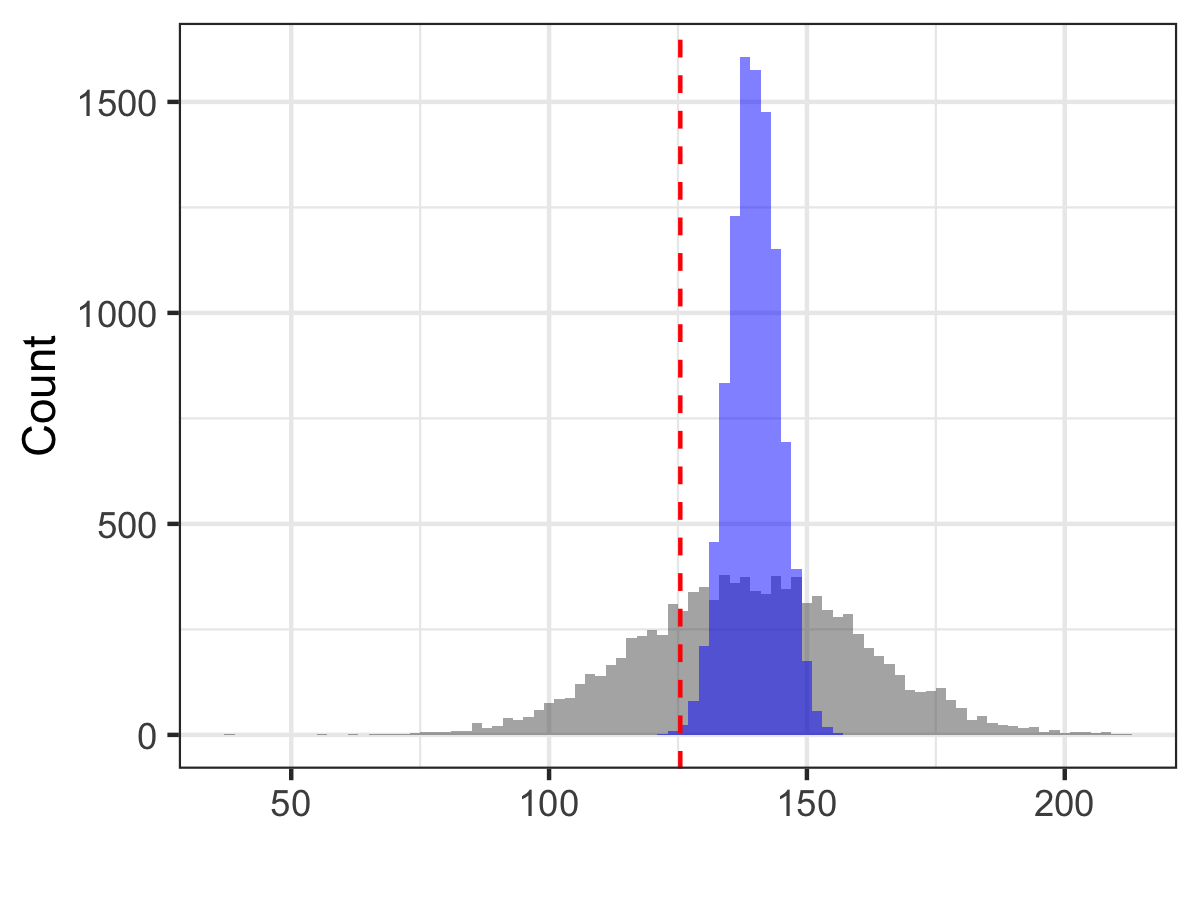
\includegraphics[width=0.7\textwidth]{img/hyp-z-test-example-2.png}
\end{center}
It turns out that the distribution of the sample mean will have the same mean, $\mu_0$, as the population distribution, but its standard deviation will be $\sigma/\sqrt{n}$, where $n$ is the number of samples over which the mean is taken.

\begin{question}{}
If $n=1$, what is the standard deviation of the sample mean? If $n=\infty$, what is the standard deviation of the sample mean?
\end{question}

\begin{question}{}
The sample mean for our $20$ sampled Appalachian men is shown as a vertical red dashed line in the figure above. Now that you know what the distribution of the sample mean looks like, do you think the observation from your Appalachian town is ``weird''?
\end{question}

\noindent Let's conduct a hypothesis test to evaluate whether we have evidence that the mean SBP among men in this town is different from that of the general U.S. population.

\begin{enumerate}
\item \textit{State the \textbf{null hypothesis}}. Here the null hypothesis is going to be our default position: that there is no difference. Let $\mu_c$ be the true mean SBP for men in the community and $\mu_0$ be the mean for the general population. 
\begin{align*}
H_0: &~\mu_c = \mu_0 \\
H_a: &~\mu_c \neq \mu_0
\end{align*}
\item \textit{List statistical {assumptions}}. We make two assumptions. First, we assume that the SBPs of the different men in the sample are statistically independent. Second, we assume that under the null, SBP will follow a normal distribution with mean 139.75 and standard deviation 21.40, the same as the general population of men aged 55-64.
\item \textit{Decide on an appropriate test and test statistic}. Our test statistic in this case is going to be the \textbf{Z-statistic}, which measures the deviation of the sample mean from the population mean in units of the standard deviation of the sample mean, $\sigma/\sqrt{n}$:
$$ Z = \frac{\overline{x} - \mu_0}{\sigma / \sqrt{n}} \qquad \text{where} \qquad \overline{x} = \frac{1}{n} \sum_{i=1}^n x^{(i)}$$
In our case, $n = 20$ because $\overline{x}$, our sample mean, is an average of 20 samples.  
\item \textit{Derive the distribution of the test statistic under the null}. The Z-statistic follows a \textbf{standard normal} distribution under the null, which is a normal distribution with $\mu=0$ and $\sigma=1$. To see this, remember that the distribution of $\overline{x}$ under the null is $\mathcal{N}(\mu_0, \sigma/\sqrt{n})$. When you calculate the Z-statistic, you shift that distribution by a distance $\mu_0$ so it is centered at zero, then adjust its width (standard deviation) to 1.0 by dividing by $\sigma/\sqrt{n}$.
\item \textit{Select a {significance level} under which you'll reject the null}. For the purposes of this example, we will choose $\alpha = 0.05$ (5\% chance of a type I error). The null distribution of the Z-statistic is shown below. The vertical dotted black lines are situated at the \textbf{critical values} that produce $\alpha = 0.05$ (the area under the null distribution that is outside those lines is 0.05). 

\begin{center}
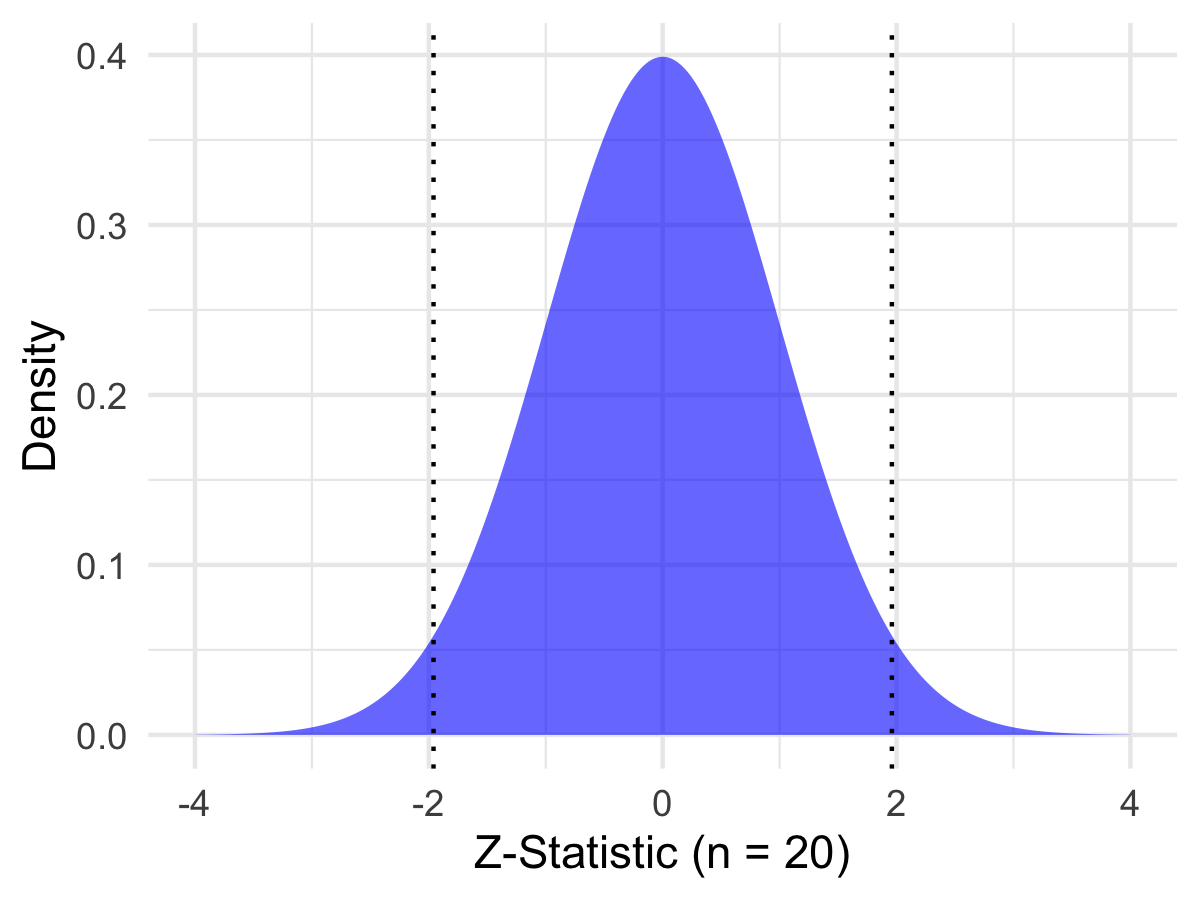
\includegraphics[width=0.7\textwidth]{img/hyp-z-test-example-3-z.png} 
\end{center}

\item \textit{Compute the observed value of the test statistic from the data.} The observed value of the test statistic is:
$$ Z = \frac{\overline{x} - \mu_0}{\sigma / \sqrt{n}} = \frac{125.45 - 139.75}{21.40/\sqrt{20}} = -2.99. $$
\item \textit{Decide whether or not to reject the null hypothesis.} The value of our test statistic falls outside the region contained by the critical values (the \textbf{acceptance region}), so we reject the null at this value of $\alpha$.
\begin{center}
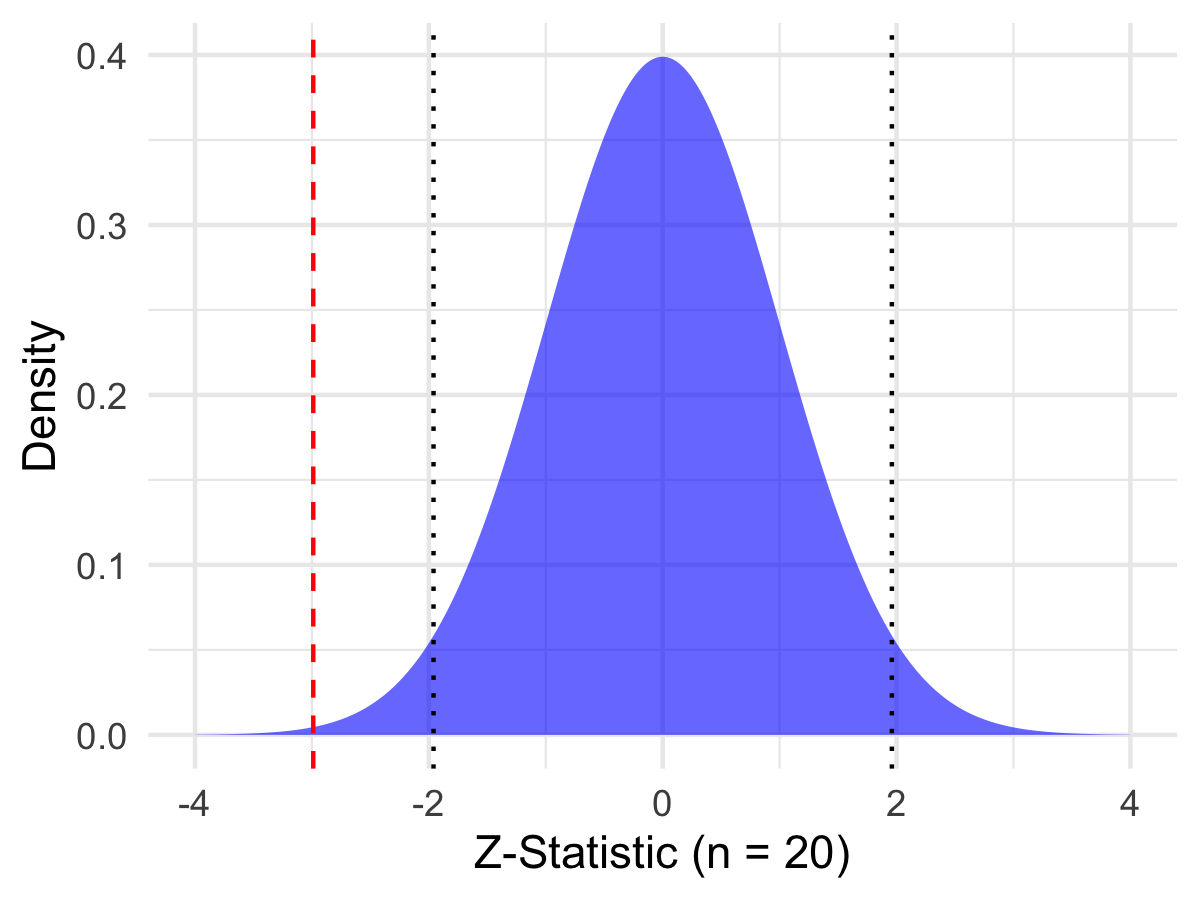
\includegraphics[width=0.7\textwidth]{img/hyp-z-test-example-4-z.png} 
\end{center}
\end{enumerate}

\begin{question}{}
As $\alpha$ gets smaller, are you more or less likely to reject the null for the same value of the test statistic? Hint: What does making $\alpha$ smaller do to the positions of the two black dotted lines in the figure, above?
\end{question}

%%%%%%%%%%%%%%%%%%%%%%%%%%%%%%%%%%%%%%%%%%%%%%%%%%%%%%%%%%%%%%%%%%%%%%%%%%%%%%%%

\section{Definitions}

\begin{itemize}
\item \textbf{Type I Error:} When a hypothesis test rejects the null even though the null is true (also called a \textbf{false positive}). The type I error rate is usually denoted by $\alpha$.
\item \textbf{Type II Error:} When a hypothesis test fails to reject the null even though it is false (also called a \textbf{false negative}). The type II error rate is usually denoted by $\beta$.
\item \textbf{P-value:} The probability of obtaining a test statistic at least as extreme as the one that was actually obtained, assuming the null is true. A $p$-value can be \textbf{one-sided} or \textbf{two-sided}. The difference lies in the definition of ``extreme''. In a one-sided test, we find the probability that the test statistic is at least as extreme \emph{in the same direction} as the one we observed. In a two-sided test, we find the probability that the test statistic is at least as extreme \emph{in either direction} (positive or negative deviation). In most cases, this has the practical effect of doubling the $p$-value.
\item \textbf{Power:} The probability that a hypothesis test will reject the null when the null is false (that the test will detect a true effect if the effect is there). Usually denoted $1 - \beta$.
\end{itemize}

%%%%%%%%%%%%%%%%%%%%%%%%%%%%%%%%%%%%%%%%%%%%%%%%%%%%%%%%%%%%%%%%%%%%%%%%%%%%%%%%

\section{Pearson's Chi-Squared Test}

Imagine you have data on two discrete variables for $n$ different subjects. You want to test whether the value of one covariate is independent of the value of the other. To do this, you can arrange your data in a \textbf{contingency table} where the rows and columns correspond to the values of the two variables. \textbf{Pearson's chi-squared test} can then be used to assess the independence of row and column values.

\paragraph{Example: Association of Genotype and Disease} Imagine you want to test whether a person's genotype at a particular locus is associated with whether or not he/she has Disease X. You find 100 people with the disease and 100 healthy controls ($n=200$) and genotype them:

\begin{center}
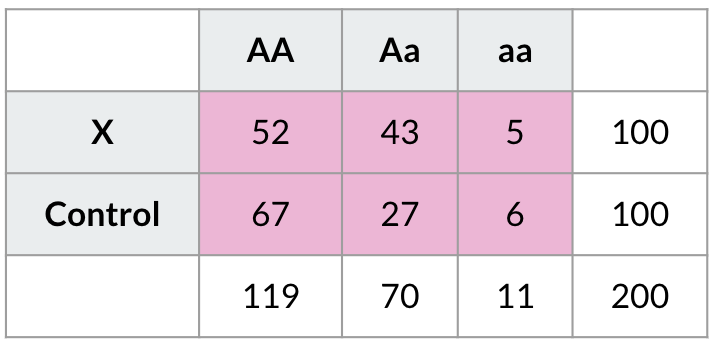
\includegraphics[width=0.55\textwidth]{img/pearson-chisq-fig-1.png}
\end{center}

\noindent \noindent Let's conduct a hypothesis test to examine this result. 

\newcommand{\indep}{\perp \!\!\! \perp}
\newcommand{\independent}{\perp\mkern-9.5mu\perp}
\newcommand{\notindependent}{\centernot{\independent}}

\begin{enumerate}
\item \textit{State the \textbf{null hypothesis}}. We consider the genotype at this locus, $G$, to be a random variable (see Chapter~\ref{chapter:probabilitydistributions}) with three possible outcomes: \emph{AA}, \emph{Aa}, and \emph{aa}. We likewise consider the patient's disease status, $D$, to be a random variable with two possible outcomes: disease or no disease. We state our null hypothesis mathematically as: 
\begin{align*}
H_0: &~ G \independent D \\
H_a: &~ G \notindependent D
\end{align*}
where the symbol $\independent$ refers to statistical independence of $G$ and $D$. We encountered statistical independence in our discussion of maximum likelihood in Chapter~\ref{chapter:mlebasics}. Mathematically, statistical independence means that the joint probability of observing a particular value for $G$ and a particular value for $D$ is simply equal to the product of their individual probabilities:
$$ P(G=g, D=d) = P(G=g) P(D=d) $$
Under these conditions, the expected values of the cells of our table are:
\begin{center}
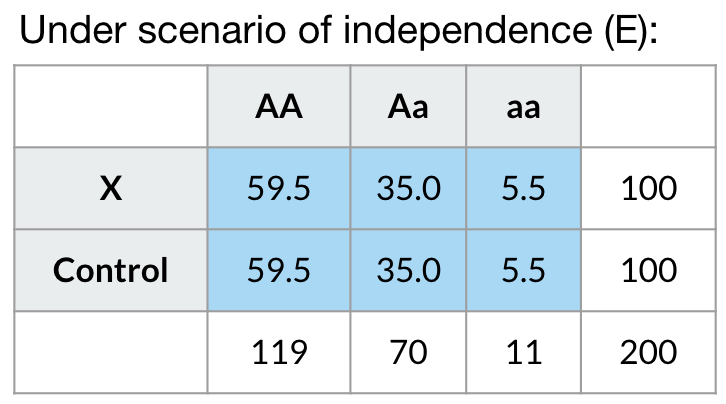
\includegraphics[width=0.55\textwidth]{img/pearson-chisq-fig-2.png}
\end{center}
For example, consider the cell $G = AA, D = X$. Assuming the total number of patients is fixed at $n=200$ and $G$ and $D$ are independent, the expected number of people in that cell is: 
\begin{align*} P(G=AA, D=X) \cdot n &= \left(\frac{119}{200}\right) \left(\frac{100}{200}\right) \cdot 200 \\
&= \mathbf{59.5} \end{align*}
Our task now is to decide whether our observed table counts are different enough from what we expect under the null to cause us to reject the null. 

\item \textit{List statistical {assumptions}}. We assume that the data are sampled randomly and independently from a fixed population where each member of the population has an equal probability of selection\footnote{A further assumption of the chi-squared test is that expected counts for each cell must be sufficiently high. A common rule is 5 or more in all cells of a $2\times 2$ table, and 5 or more in 80\% of cells in larger tables, but no cells with zero counts.}. 

\item \textit{Decide on an appropriate test and test statistic}. The chi-squared test works by calculating expected counts in all $r \times c$ cells of the table ($r$ = number of rows, $c$ = number of columns) and then measuring the data's deviation from those expected counts. The \textbf{chi-squared test statistic} has the form
$$ X^2 = \sum_{i=1}^r \sum_{j=1}^c \frac{(O_{ij} - E_{ij})^2}{E_{ij}} $$
where $O$ refers to ``observed count'' and $E$ to ``expected count''. The expected counts are those that assume statistical independence of rows and columns (blue table, above).

\item \textit{Derive the distribution of the test statistic under the null}. Under the null, the $X^2$ test statistic follows a chi-squared distribution (Section~\ref{sect:chisqdist}) with $(r-1)(c-1)$ degrees of freedom. In the case of our genotype example, there are $r=2$ rows and $c=3$ columns, thus $2$ degrees of freedom.

\item \textit{Select a {significance level} under which you'll reject the null}. The $\chi^2$ distribution with $2$ degrees of freedom is shown below. Two vertical lines are shown at different significance levels: $\alpha = 0.05$ and $\alpha = 0.1$.

\begin{center}
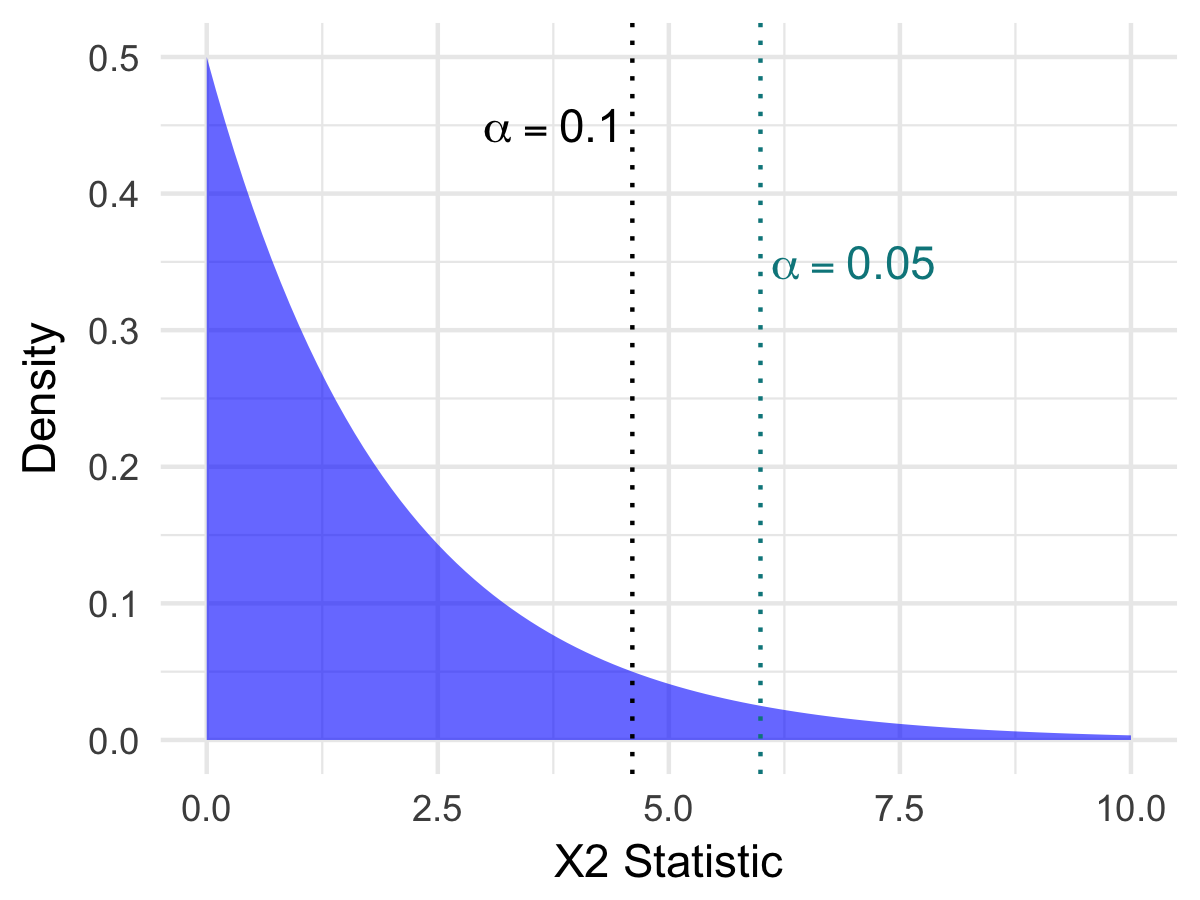
\includegraphics[width=0.6\textwidth]{img/hyp-chisq-test-example-2.png} 
\end{center}

\item \textit{Compute the observed value of the test statistic from the data.}

\begin{question}{}
Using the formula in step~$4$, above, compute the actual value of the chi-squared test statistic for this example. Hint: You should end up with a value that corresponds to the position of the red dashed line in the figure below. 
\begin{center}
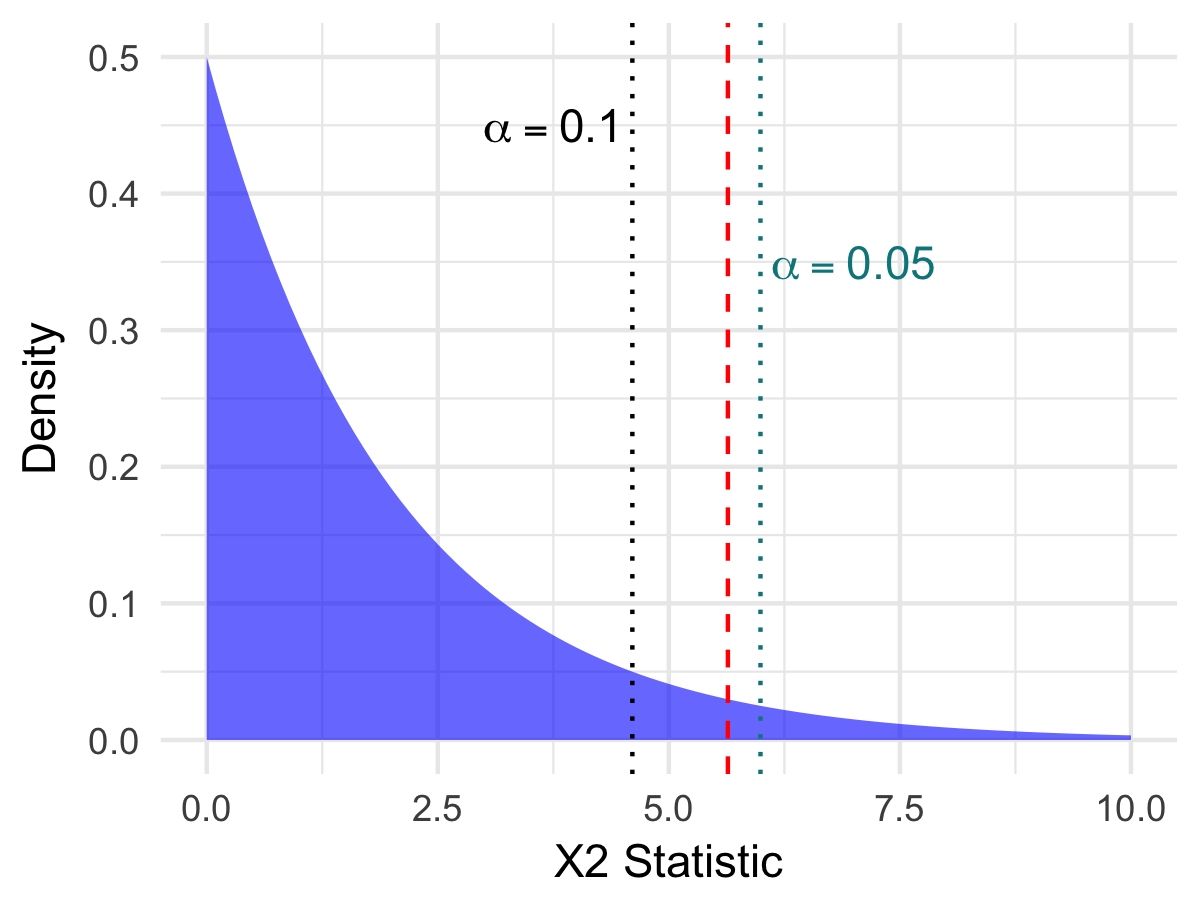
\includegraphics[width=0.7\textwidth]{img/hyp-chisq-test-example-3.png} 
\end{center}
\end{question}

\item \textit{Decide whether or not to reject the null hypothesis.} Based on our calculated value of the test statistic, we will reject the null at $\alpha = 0.1$ and fail to reject the null at $\alpha = 0.05$.
\end{enumerate}

Although it looks much different from the Z-test, the chi-squared test follows the same formalism: defining a null hypothesis, figuring out what the data should look like under the null, quantifying the deviation of the observed data from what's expected using a test statistic, and deciding if that test statistic presents strong enough evidence to cause us to reject the null.  

%%%%%%%%%%%%%%%%%%%%%%%%%%%%%%%%%%%%%%%%%%%%%%%%%%%%%%%%%%%%%%%%%%%%%%%%%%%%%%%%%%%%%%

\section{Student's T-tests}

The final example we will look at today is the \textbf{T-test}. Like the $Z$-test, the $T$-test (actually a family of tests) deals with situations where you have data that are assumed to be normally distributed under the null hypothesis. However, in this scenario, the population standard deviation, $\sigma$ is not known and must be estimated from the data itself.

\subsection{One Sample T-test}

Assume you have a dataset $x^{(1)}, \dots, x^{(n)}$, of real numbers that you can plausibly assume are normally distributed. You want to test whether the mean of your data is equal to a fixed value, $\mu_0$. Under the null hypothesis that the means are the same, the test statistic
$$ T = \frac{\overline{x} - \mu_0}{s/\sqrt{n}} $$
which we call a ``T statistic'', follows a T-distribution (Section~\ref{sect:tdist}) with $n-1$ degrees of freedom\footnote{A one-sample T-test looks a lot like a Z-test. However, because we use $s$ to estimate the population standard deviation from data, we must account for variation in our estimate. It turns out that the sample variance, $s^2$, follows a chi-squared distribution with $n-1$ degrees of freedom, where $n$ is the sample size. In this case, by the definition of the $T$-distribution (Section~\ref{sect:tdist}), the T statistic follows a Student's T-distribution with $n-1$ degrees of freedom. As the number of samples, $n$, grows, the sample standard deviation approaches the population standard deviation and the T-test becomes a Z-test. But when $n$ is small, the T-test is quite a bit more conservative.}. Here $\overline{x}$ refers to the sample mean, and $s$ refers to the \textbf{sample standard deviation}:
$$ s = \sqrt{\frac{1}{n-1} \sum_{i=1}^n (x^{(i)} - \overline{x})^2} $$

\begin{question}{}
Compare the formula for the sample standard deviation to the maximum likelihood estimate of the parameter, $\sigma$, of a normal distribution (Section~\ref{sect:mlenormal}). What is the same/different? Note in particular the use of $n-1$ in the denominator, rather than $n$. This arises because the MLE for $\sigma$, $\hat{\sigma}$, is a \textbf{biased} estimate of the population standard deviation (more on this later). For large $n$, however, the two are nearly identical. 
\end{question}

\subsection{Two Independent Samples, Equal Variance}

Assume you have a dataset $x^{(1)}, \dots, x^{(n)}$ and another dataset $y^{(1)}, \dots, y^{(m)}$. You assume that both are drawn from normal distributions with equal variance but potentially different means. You want to test whether the means are equal. 

The same basic machinery for the one-sample T-test can be deployed in this context with a slightly different test statistic. The test statistic
$$ T = \frac{\overline{x} - \overline{y}}{s_p \sqrt{\cfrac{1}{n} + \cfrac{1}{m}}} $$
where
\begin{align*} s_p^2 &= \frac{(n-1) s_x^2 + (m-1) s_y^2}{m + n - 2} \\
s_x^2 &= \frac{1}{n-1} \sum_{i=1}^n (x^{(i)} - \overline{x})^2 \\
s_y^2 &= \frac{1}{m-1} \sum_{i=1}^m (y^{(i)} - \overline{y})^2 \end{align*}
follows a $t$-distribution with $m + n - 2$ degrees of freedom.

\subsection{Two Independent Samples, Unequal Variance}

Sometimes you have two independent samples but cannot assume the variances are equal. Again, similar machinery can be deployed. In this case, you can use \textbf{Welch's T-test}, which uses the test statistic
$$ T = \frac{\overline{x} - \overline{y}}{s_{xy}} $$
where 
$$ s_{xy} = \sqrt{\frac{s_x^2}{n} + \frac{s_y^2}{m}}. $$
This test statistic approximately follows a $t$-distribution with degrees of freedom given by the {Welch-Sattherwaite Equation}
$$ \text{d.f.} = \frac{\left(\cfrac{s_x^2}{n} + \cfrac{s_y^2}{m} \right)^2}{\cfrac{(s_x^2/n)^2}{n-1} + \cfrac{(s_y^2/m)^2}{m-1}} $$ 

\subsection{Matched Pairs}

Assume you have a data set of matched pairs. This could be a set of measurements of the same individuals taken at two different points in time, for example, or paired measurements taken from individuals with similar characteristics. You want to test whether the second set of values have changed relative to the first set of values.

To do this, you can use a one-sample T-test on the \emph{differences} of the individual pairs. If no change has occurred, you would expect the mean of those differences to be zero. If we define $x^{(i)}$ as the difference of the paired observations for sample $i$ and $\overline{x}$ as $\frac{1}{n}\sum_{i=1}^n x^{(i)}$, the sample mean of those differences, then

$$ T = \frac{\overline{x}}{s/\sqrt{n}}$$

\noindent follows a T-distribution with $n-1$ degrees of freedom. 

\begin{question}{}
Here are some sample data. They come from a study that looked at the effect of ozone, a component of smog, on the weight gain of rats. (Original source: Biometrika 63: 421-434, 1976, reproduced in Rice's \emph{Mathematical Statistics and Data Analysis}, p. 465.) A group of 22 seventy-day-old rats were kept in an environment containing ozone for $7$ days, and their weight gains were recorded. Another group of 23 rats of a similar age were kept in an ozone-free environment for a similar time and their weight gains were also recorded. Here are the data for the control group:

{\footnotesize \tt
\begin{center}
\begin{tabular}{rlrr}
  \toprule
  & group & original\_weight & weight\_gain \\ 
  \midrule
  1 & control & 340.8 & 41.0 \\ 
  2 & control & 389.1 & 25.9 \\ 
  3 & control & 355.2 & 13.1 \\ 
  4 & control & 421.8 & -16.9 \\ 
  5 & control & 377.1 & 15.4 \\ 
  6 & control & 404.3 & 22.4 \\ 
  7 & control & 321.2 & 29.4 \\ 
  8 & control & 447.5 & 26.0 \\ 
  9 & control & 305.9 & 38.4 \\ 
  10 & control & 335.9 & 21.9 \\ 
  11 & control & 386.3 & 27.3 \\ 
  12 & control & 377.0 & 17.4 \\ 
  13 & control & 357.2 & 27.4 \\ 
  14 & control & 441.7 & 17.7 \\ 
  15 & control & 383.7 & 21.4 \\ 
  16 & control & 373.7 & 26.6 \\ 
  17 & control & 336.0 & 24.9 \\ 
  18 & control & 419.4 & 18.3 \\ 
  19 & control & 287.1 & 28.5 \\ 
  20 & control & 602.8 & 21.8 \\ 
  21 & control & 325.4 & 19.2 \\ 
  22 & control & 452.4 & 26.0 \\ 
  23 & control & 398.9 & 22.7 \\ 
  \midrule
  Mean & control & 384.4 & 22.4 \\
  St.Dev. & control & 65.5 & 10.8 \\
  \bottomrule
\end{tabular}
\end{center}
}

\noindent And here are the data for the ozone group:

{\footnotesize \tt
\begin{center}
\begin{tabular}{rlrr}
  \toprule
  & group & original\_weight & weight\_gain \\ 
  \midrule
  1 & ozone & 437.4 & 10.1 \\ 
  2 & ozone & 275.9 & 7.3 \\ 
  3 & ozone & 296.3 & -9.9 \\ 
  4 & ozone & 295.9 & 17.9 \\ 
  5 & ozone & 379.7 & 6.6 \\ 
  6 & ozone & 274.1 & 39.9 \\ 
  7 & ozone & 360.0 & -14.7 \\ 
  8 & ozone & 331.9 & -9.0 \\ 
  9 & ozone & 531.8 & 6.1 \\ 
  10 & ozone & 350.5 & 14.3 \\ 
  11 & ozone & 345.7 & 6.8 \\ 
  12 & ozone & 268.1 & -12.9 \\ 
  13 & ozone & 339.9 & 12.1 \\ 
  14 & ozone & 352.4 & -15.9 \\ 
  15 & ozone & 435.8 & 44.1 \\ 
  16 & ozone & 476.9 & 20.4 \\ 
  17 & ozone & 462.5 & 15.5 \\ 
  18 & ozone & 368.0 & 28.2 \\ 
  19 & ozone & 504.3 & 14.0 \\ 
  20 & ozone & 188.0 & 15.7 \\ 
  21 & ozone & 466.9 & 54.6 \\ 
  22 & ozone & 288.8 & -9.0 \\ 
  \midrule
  Mean & ozone & 365.0 & 11.0 \\
  St.Dev. & ozone & 88.6 & 19.0 \\
  \bottomrule
\end{tabular}
\end{center}
}

\begin{enumerate}
\item[(a)] Imagine that the population weight distribution of rats is known to be normal with $\mu = 350$ (grams) and unknown $\sigma$. How would you test the hypothesis that the mean of the control group is equal to the population mean? How would you test the hypothesis that the mean of the ozone group is equal to the population mean?
\item[(b)] How would you test the hypothesis that the mean original weights of the ozone and control groups are equal? Do not assume equal variance. 
\item[(c)] How would you test the hypothesis that the mean weight gain in the ozone group is equal to the mean weight gain in the control group? Do not assume equal variance.
\item[(d)] How would your approach in part (c) change if you assumed the weight gains in the two groups had equal variance?
\end{enumerate}

\noindent Plug in the relevant numbers from the tables above to perform each hypothesis test with $\alpha = 0.05$. The following table of critical values for the $T$-distribution\footnote{Borrowed with gratitude from https://www.stat.purdue.edu/~lfindsen/stat503/t-Dist.pdf} may help you:

\begin{center}
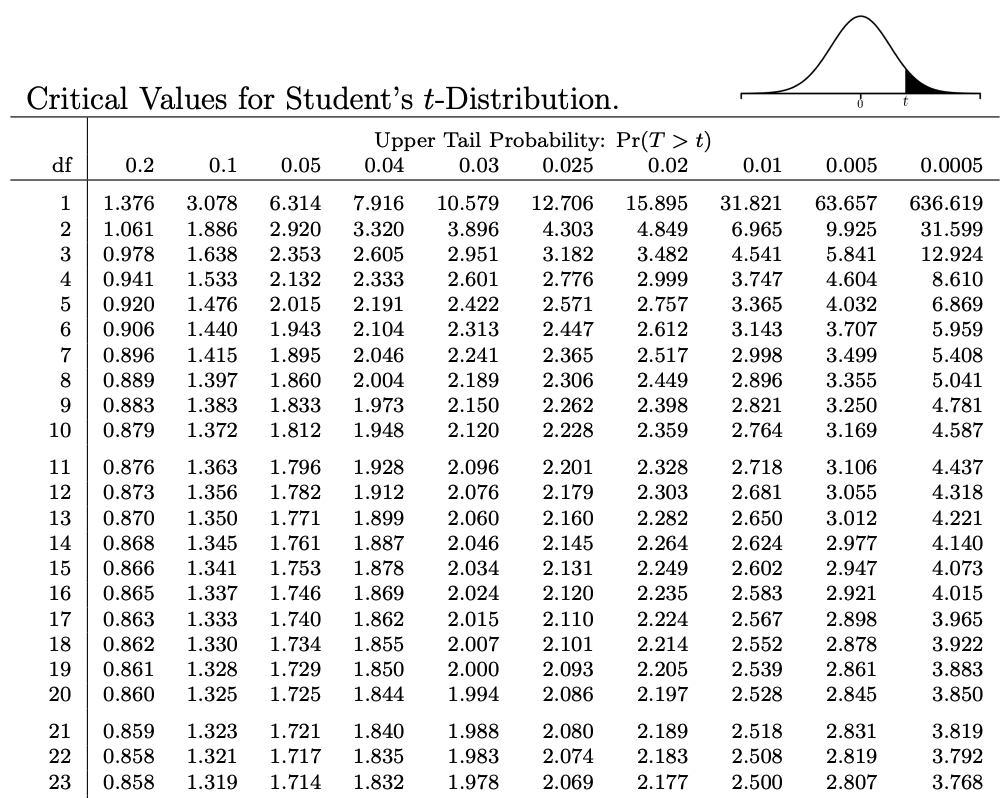
\includegraphics[width=0.9\textwidth]{img/t-distribution-critical-values.png}
\end{center}

\noindent \textbf{Answers:} (a) One-sample $T$-test of control group original weights vs. null of $\mu_0 = 350$; $T$-statistic is 2.5165, 22 d.f., two-sided $p$-value is 0.01964, reject null at $\alpha=0.05$. One-sample $T$-test of ozone group original weights vs. null of $\mu_0 = 350$; $T$-statistic is 0.7961, 21 d.f., two-sided $p$-value is 0.4349, fail to reject null at $\alpha=0.05$. (b) Welch's two-sample $T$-test of control vs. ozone group original weights; $T$-statistic is 0.8293, d.f is estimated using the Welch-Sattherwaite equation at 38.619, two-sided $p$-value is 0.4120, fail to reject null at $\alpha=0.05$. (c) Welch's two-sample $T$-test of control vs. ozone group weight gains; $T$-statistic is 2.4629, d.f. is estimated using the Welch-Sattherwaite equation at 32.918, two-sided $p$-value is 0.01918, reject null at $\alpha=0.05$. (d) You would use Pearson's two-sample $T$-test, which assumes equal variances; $T$-statistic is 2.4919, d.f. is 43, two-sided $p$-value is 0.01664, reject null at $\alpha=0.05$. 

\end{question}
